\documentclass[t]{beamer}

% Load general definitions
\input{../Campelo/defs/preamble.tex}

% Specific definitions
\title[]{COMP320 Research Practice}
\subtitle[]{04 - Experimentation and Hypotheses}
\date[]{}

\begin{document}

% cover page
\setbeamertemplate{footline}{}
\begin{frame}
  \titlepage
\end{frame}

%=====

% Main slides
\begin{ftst}
{Experiments}
{Definition of experiment}
\vone
\begin{colorblock}{}{bg=green!30,fg=black}
\begin{center}
\textit{An experiment can be characterized as a test (or a series of tests) wherein changes are introduced in the state of a system or process, enabling the observation and characterization of effects that can occur as a result of these changes.}
\end{center}
\end{colorblock}
\vone
Usually performed with an objective in mind:

\bitems Uncovering influential variables in a given system or process;
	\spitem Determining desired values for certain parameters
	\spitem Characterize behavior of the system or process under study.
\eitem
\end{ftst}

%=====

\begin{ftst}
{Experiments}
{Data gathering}
\begin{block}{}
	{\small\bitems\alert{Retrospective study};
		\item Observational study;
		\item Designed experiment;
	\eitem}
\end{block}
\begin{block}{Characteristics}
	{\small\bitems Use of historical data;
	\item Investigating correlations;\eitem
	}
\end{block}
\begin{block}{Problems}
	{\small\bitems Data representativeness;
	\item Availability of data;\eitem
	}
\end{block}
\end{ftst}

%=====

\begin{ftst}
{Experiments}
{Data gathering}
\begin{block}{}
	{\small\bitems Retrospective study;
		\item \alert{Observational study};
		\item Designed experiment;
	\eitem}
\end{block}
\begin{block}{Characteristics}
	{\small\bitems Observation of the system with minimal disturbance;
	\item Investigation of usual behaviors;\eitem
	}
\end{block}
\begin{block}{Problems}
	{\small\bitems Low representativeness of extreme cases;
	\item Low variability can affect observation of interesting effects;\eitem
	}
\end{block}
\end{ftst}

%=====

\begin{ftst}
{Experiments}
{Data gathering}
\begin{block}{}
	{\small\bitems Retrospective study;
		\item Observational study;
		\item \alert{Designed experiment};
	\eitem}
\end{block}
\begin{block}{Characteristics}
	{\small\bitems Introduction of deliberate changes in the system;
		\item Inference on the \textit{causality} of the effects;
		\eitem}
\end{block}
\begin{block}{Problems}
	{\small\bitems Requires rigorous experimental design and data analysis;
	\item Usually more expensive.
	\eitem}
\end{block}
\end{ftst}

%=====

\begin{ftst}
{Experimentation strategies}
{Educated guessing}
\vspace{-1em}
\begin{columns}[T]
\column{1.02\textwidth}
	\begin{block}{}
		\bitems Select arbitrary combination of levels for the factors;
			\item Test and observe behavior; 
			\item Change one or two factors at a time, then re-test;
		\eitem
	\end{block}
\bitems Widely used in industry;
\item Can achieve good results, but has a lot of limitations;
\eitem
\end{columns}
\end{ftst}

%=====

\begin{ftst}
{Experimentation strategies}
{COST: Change One Separate factor at a Time}
\begin{columns}[T]
\column{1.02\textwidth}
	\begin{block}{}
		\bitems Select a reference point;
			\item Change each factor individually, keeping all others constant;
		\eitem
	\end{block}
	\vone
	\bitems Also widely used;
		\item Can achieve good results as long as there are no interaction effects;
	\eitem
\end{columns}
\begin{tikzpicture}[remember picture,overlay]
	\node[anchor=south east,yshift=0pt, xshift=-5pt] at (current page.south east) {\includegraphics[width=5.5cm]{../Campelo/figs/OFAT01c.png}};
\end{tikzpicture}
\lfr{Image: (c) D.C. Montgomery}
\end{ftst}

%=====

\begin{ftst}
{Experimentation strategies}
{Factorial designs}
\begin{columns}[T]
\column{1.02\textwidth}
	\begin{block}{}
		\bitems Select \textbf{levels} for each factor;
			\item Vary the factors simultaneously, in a systematic way;
		\eitem
	\end{block}
	\bitems Estimation of main effects and interactions;
		\item Greater precision in the effect estimates;
		\item More efficient use of resources (information/observation);
	\eitem
\end{columns}
\begin{tikzpicture}[remember picture,overlay]
	\node[anchor=south east,yshift=0pt, xshift=-5pt] at (current page.south east) {\includegraphics[width=5.5cm]{../Campelo/figs/FFD01a.png}};
\end{tikzpicture}
\lfr{Image: (c) D.C. Montgomery}
\end{ftst}

%=====

\begin{ftst}
{Fundamental principles}
{Design of experiments (DoE)}
\vone
\begin{colorblock}{}{bg=green!30,fg=black}
\begin{center}
\textit{Process of designing data gathering protocols to enable\\
accurate analyses by statistical tools, capable of supporting\\
sound and objective conclusions.}
\end{center}
\end{colorblock}

\bitems Applicable to systems and processes subject to noise, experimental errors, uncertainties, etc.
	\item Necessary for the conclusions to have a quantifiable meaning;
	\item Helpful in avoiding errors due to personal biases or other artifacts of experimentation and analysis.
\eitem
\end{ftst}

%=====

\begin{ftst}
{Fundamental principles}
{Design of experiments (DoE)}
\begin{block}{Design of the experiment}
	\small
	\bitems Scientific/technical question of interest;
		\item Selection of variables and values;
		\item Definition of the desired confidence level;
		\item Sample size calculations;
		\item Determination of protocols for data gathering;
	\eitem
\end{block}
\begin{block}{Statistical analyses of the data}
	\small
	\bitems Calculation of a test statistic;
		\item Validation of the assumptions of the statistical model;
		\item Calculation of the magnitude of effects;
		\item Drawing of conclusions and recommendations;
	\eitem
\end{block}
\end{ftst}

%=====

\begin{ftst}
{Fundamental principles}
{Design of experiments (DoE)}
\begin{block}{}
	\bitems \alert{Repetition and replication};
		\item Randomization;
		\item Blocking.
	\eitem
\end{block}
	\bitems Repeated measurements - estimation of within-group variability;
		\item Replication - estimative of the experimental error;
		\item Greater precision in estimating the model parameters;
	\eitem
\end{ftst}

%=====

\begin{ftst}
{Fundamental principles}
{Design of experiments (DoE)}
\begin{block}{}
	\bitems Repetition and replication;
		\item \alert{Randomization};
		\item Blocking;
	\eitem
\end{block}
\bitems Avoids contamination of the data by order-dependent effects such as:

	\bitems Heating effects;
		\spitem Wear and tear effects;
		\spitem External interferences;
	\eitem
\eitem
\end{ftst}

%=====

\begin{ftst}
{Fundamental principles}
{Design of experiments (DoE)}
\begin{block}{}
	\bitems Repetition and replication;
		\item Randomization;
		\item \alert{Blocking};
	\eitem
\end{block}
\bitems Isolation of nuisance variables (those that influence the response, but are not interesting for the analyses) that can be controlled;
	\spitem Improvement in the estimation of effects for the factors of interest;
	\spitem Reduction or eliminations of inconvenient factor effects;
\eitem
\end{ftst}

%=====

\begin{ftst}
{Fundamental principles}
{The role of experimental design}
Experimental design is useful for avoiding the influence of spurious factors and personal biases on the results, by performing experiments in a impartial and objective way.
\begin{colorblock}{}{bg=green!30,fg=black}
	\vhalf
	\centering``\textit{Never have too much love for your hypotheses.}''
	\vspace{0.5em}
\end{colorblock}
\vone
\begin{columns}[T] 
\column{0.7\textwidth}
	\begin{colorblock}{}{bg=green!30,fg=black}
		\flushright{``\textit{The great tragedy of Science - the slaying of a\\
		\vspace{-1em}\flushright beautiful hypothesis by an ugly fact.}''\\
		-- Thomas H. Huxley}
		\vspace{0.5em}
	\end{colorblock}
\column{0.3\textwidth}
\end{columns}
\begin{tikzpicture}[remember picture,overlay]
	\node[anchor=south east,yshift=20pt, xshift=-10pt] at (current page.south east) {\includegraphics[width=2.5cm]{../Campelo/figs/huxley.png}};
\end{tikzpicture}
\lfr{Image: \url{http://www.iep.utm.edu/huxley/}}
\end{ftst}

%=====

\begin{ftst}
{Discussion}
{Jacques Benveniste and the memory of water}
\begin{columns}
\column[T]{0.85\textwidth}
	\bitems Nature (1988);
		\item Investigation committee: Maddox, Stewart, Randi;
		\item Retracted by Nature due to evidence of misconduct.
	\eitem
\column[T]{0.15\textwidth}
	\begin{tikzpicture}[remember picture,overlay]
		\node[anchor=north east,yshift=-50pt, xshift=-10pt] at (current page.north east) {\includegraphics[width=1.1\textwidth]{../Campelo/figs/benveniste.png}};
	\end{tikzpicture}
\end{columns}
\vone
\begin{columns}
\column[T]{0.8\textwidth}
	\begin{block}{Methodological problems}
	\small
	\bitems Experimenter bias (absence of proper blinding);
		\item Cherrypicking (selective recording of results);
		\item Unaccounted sampling errors;
		\item Possible contamination;
		\item Complete lack of prior physical/ chemical plausibility;
		\item \textbf{Non-reproducibility}.
	\eitem
\end{block}
\column[T]{0.2\textwidth}
\end{columns}
\lfr{Image: \url{http://www.jacques-benveniste.org/inmemoriam/photo1.html}}
\end{ftst}

%=====

\begin{ftst}
{Structure of Experimental Design}
{Guidelines for a good design}
\bitems Pre-experimental design:

	\bitems Identification and definition of the problem;
		\spitem Selection of experimental and response variables of interest;
		\spitem Choice of experimental protocols;
	\eitem
	\spitem Choice of the experimental design;
	\spitem Collection of the data;
	\spitem Statistical data analyses;
	\spitem Conclusions and recommendations;
\eitem
\end{ftst}

%=====

\begin{ftst}
{Pre-experimental design}
{Before we start}
\bitems Is the investigation relevant?
	\spitem Would the results be interesting for the research community?
	\spitem Practical relevance?
	\bitems Employ exploratory experiments;\eitem
	\spitem Placement within the literature;
	\bitems Avoid repetition and irrelevance.\eitem
\eitem
\end{ftst}

%=====

\begin{ftst}
{Pre-experimental design}
{Definition of hypotheses}
\bitems The translation \textit{scientific question} $\rightarrow$ \textit{test hypothesis} requires special attention, and a solid knowledge of the technical area in which the experiment is being performed;
\eitem
\end{ftst}

%=====

\begin{ftst}
{Actual Experiment}
{Data gathering}
\bitems Must be consistent with design, otherwise the validity of the results may be compromised - data collection must always follow the plan:\vhalf
	\bitems No premature stops;	
		\spitem\textit{No-peeking rule} (except when planned, of course);
	\eitem
	\spitem Use of pilot experiments:\vhalf
	\bitems Gathering of preliminary information;
		\spitem Practice with the experimental conditions;
	\eitem
\eitem
\end{ftst}

%=====

\begin{ftst}
{Analysis of the experimental data}
{Statistical modeling}
\bitems General procedure for testing the experimental hypotheses:

	\bitems Definition of a \textit{null-model} (absence of effects) and of a desired level of significance;
		\spitem Determination of $P(data|\mbox{\textit{null-model}})$;
		\spitem Decision by rejection (or not) of the null hypothesis;
		\spitem Validation of model assumptions;
		\spitem Estimation of the  \textit{magnitude} of differences - \textbf{practical significance};
	\eitem
\eitem

\begin{block}{}
	\centering\textit{Statistical methods do not \textbf{prove} anything, but they allow an objective definition of margins of plausibility for certain statements.}
\end{block}
\end{ftst}

%=====

\begin{ftst}
{Reporting of results}
{Presentation}
Combine textual, numeric and graphical elements to tell a story with your data. It simplifies the understanding and analysis of the results.
\begin{columns}[T]
\column{0.75\textwidth}
	\bitems Strive to achieve graphical excellence;
		\spitem Coherence of notation - special attention to figures and tables;
		\spitem Display simultaneous confidence intervals and other graphical indicators of effect size.
	\eitem
\column{0.25\textwidth}
	\centering\includegraphics[height=2.5cm]{../Campelo/figs/tufte.jpg}\\
	\vone
	\centering\includegraphics[height=2.5cm]{../Campelo/figs/yau.png}
\end{columns}
\lfr{Other great resources on graphical excellence:}
\lfr{\textit{Flowing Data} (\url{http://flowingdata.com/})}
\lfr{\textit{Information is Beautiful} (\url{http://www.informationisbeautiful.net})}
\end{ftst}

\begin{ftst}
{Conclusions}
{Drawing and reporting conclusions}
\bitems Conclusions should be based on solid evidence from the data;
	\spitem Be conservative - it is common to exaggerate the generality of the results;
	\spitem Report significance levels and the assumptions under which the results are valid;
	\spitem \textit{Suggest explanations} to the observed results;
	\spitem Careful with \textit{anomaly hunting};
\eitem

\begin{colorblock}{}{bg=green!30,fg=black}
	\small\textit{Always let the science drive the statistics. If you get a statistically significant result, go back and describe what it means in the scientific context.}
	\flushright\small -- Aaron Rendahl
\end{colorblock}
\end{ftst}



\begin{ftst}
{Bibliography}
{\ }
\scriptsize

\benums Dept. Biochemistry \& Cell Biology, Rice University , \textit{Common Errors in Student Research Papers.} - {\tiny\url{http://www.ruf.rice.edu/~bioslabs/tools/report/reporterror.html}}
\item T. Brady, \textit{Reviewer's quick guide to common statistical errors in scientific papers.}\\
{\tiny\url{https://goo.gl/IKvAYc}}
\item R.M. Szydloa et al., \textit{Sign of the Zodiac as a predictor of survival for recipients of an allogeneic stem cell transplant for chronic myeloid leukaemia (CML): an artificial association.} Transplantation Proceedings 42 (8):3312-3315, 2010.
\item D.C. Montgomery, \textit{Design and Analysis of Experiments}, Chapter 1. 5th ed., Wiley, 2005

\item S.C. Stearns, \textit{Some Modest Advice for Graduate Students} - {\tiny\url{http://goo.gl/jtT4hA}}
\item A. Rendahl, \textit{Experimental design and statistical analysis: questions to consider as you write your grant.} - {\tiny\url{http://goo.gl/yT0TK7}}
\item J. Maddox et al., \textit{``High-dilution'' experiments a delusion.} Nature 334, 287-290, 1988
\item V. Czitron, \textit{One-Factor-at-a-Time Versus Designed Experiments.} The American Statistician, 53(2) 126-131, 1999.
\item B. Dunning, \textit{An Enthusiast's Primer on Study Types}. Skeptoid Podcast, Skeptoid Media, Inc., 2013. - 
{\tiny\url{http://skeptoid.com/episodes/4381}}

\eenum
\end{ftst}

%=====

% Main slides
\begin{ftst}
{Statistical hypotheses}
{Scientific Hypotheses}
A \textit{hypothesis} is a proposed explanation for an observable phenomenon.
\vone
Scientific hypotheses must satisfy (at least) two conditions:

\bitems Falsifiability;
	\item Testability;
\eitem
\vone
\begin{columns}[T]
    \column{0.75\textwidth}
	\begin{colorblock}{}{bg=green!30,fg=black}
	``\textit{The more we learn about the world, and the deeper\\
	our learning, the more conscious, specific,\\
	and articulate will be our knowledge of what\\
	we do not know, our knowledge of our ignorance.}''\\
	\flushright\vspace{-1em}\small Sir Karl R. Popper\\
	\flushright\vspace{-1em}\small (1902-1994)\\
	\flushright\vspace{-1em}\small Austro-British philosopher
	\end{colorblock}
	\column{0.25\textwidth}
\begin{tikzpicture}[remember picture,overlay]
\node[anchor=south east,yshift=13pt,xshift=0pt] at (current page.south east) {\includegraphics[width=\textwidth]{../Campelo/figs/popper.png}};
%\node[anchor=south east,yshift=0pt,xshift=-15pt] at (current page.south east) {Karl Popper};
\end{tikzpicture}
\end{columns}
\lfr{Image: Copyright 2008 Ivan Jer\^onimo \url{http://www.ivanjeronimo.com.br}}
\end{ftst}

%=====

\begin{ftst}
{Statistical Hypothesis}
{The hypothetico-deductive model}
The \textit{hypothetico-deductive model} of construction of scientific knowledge includes:

\bitems Formulation of falsifiable hypotheses;
	\item Refutation or corroboration of the hypotheses by the data;
	\item Comparison between alternative hypotheses - principle of parsimony (Ockham's razor);
	\item Predictive power;
\eitem

\begin{columns}[T]
	\column{0.20\textwidth}
\begin{tikzpicture}[remember picture,overlay]
\node[anchor=south west,yshift=20pt,xshift=15pt] at (current page.south west) {\includegraphics[width=.7\textwidth]{../Campelo/figs/ockham2.png}};
\end{tikzpicture}
    \column{0.80\textwidth}
    \vhalf
	\begin{colorblock}{}{bg=green!30,fg=black}
	``\textit{Numquam ponenda est pluralitas sine necessitate.}''\\
	\flushright\vspace{-1em}\small William of Ockham\\
	\flushright\vspace{-1em}\small (1287-1347)\\
	\flushright\vspace{-1em}\small English philosopher and theologian\\
	\end{colorblock}
\end{columns}
\lfr{Image: \url{http://www.philosophybasics.com/philosophers_ockham.html}}
\end{ftst}


%=====

\begin{ftst}
{Statistical Hypotheses}
{Definitions}
\textit{Statistical hypotheses} are defined as objective statements about parameters of one ore more populations;
\vone
\textbf{Attention}: the statements in statistical hypotheses are about parameters of the \textit{population} or \textit{model}, \textbf{not the \textit{sample}}.
\vone
On frequentist approaches, the formal test of hypotheses involves the contrast between \textit{null} and \textit{alternative} hypotheses.
\begin{columns}[T]
	\column{0.48\textwidth}
	\begin{block}{Null hypothesis ($H_0$)}
	\small
	\bitems Absence of effects;
	\item \textit{Conservative} model.\eitem
	\textbf{Example:} $H_0: \mu = 25$
	\end{block}
	\column{0.48\textwidth}
	\begin{block}{Alternative hypothesis ($H_1$)}
	\small 
	\bitems Presence of some effect;
	\item Existence of something ``new''.\eitem
	\textbf{Example:} $H_1: \mu \neq 25$
		\end{block}
	\end{columns}
\end{ftst}

%=====

\begin{ftst}
{Statistical Hypotheses}
{Example}
Suppose you own a company that sells green peas to large customers, 
and that you want to determine whether your $50$kg sacks really 
contain their nominal weight (at least on average).
\vhalf
In this case the null hypothesis could be defined as:
\textit{the average net weight of a sack is $50$kg}, and the alternative of interest could be expressed as the complementary inequality.
\beqs\begin{cases}
H_0: \mu = 50kg \\
H_1: \mu \neq 50kg 
\end{cases}\eqs
\vone
Suppose still that $n = 10$ packs are randomly sampled, and their contents are weighted using a calibrated scale;
\begin{tikzpicture}[remember picture,overlay]
\node[anchor=north east,yshift=12pt,xshift=-5pt] at (current page.north east) {\includegraphics[width=0.2\textwidth]{../Campelo/figs/peas.png}};
\end{tikzpicture}
\lfr{Image: \url{http://www.storko.eu/ed_files/image/green-peas.jpg}}
\end{ftst}

%=====

\begin{ftst}
{Statistical Hypotheses}
{Example}
Since the sample mean $\bar{x}$ is a good estimator of the real mean $\mu$, common sense suggests that:

\bitems If $\bar{x} \cong 50$kg - corroboration of $H_0$;
\item If $\bar{x} \ll 50$kg or $\bar{x} \gg 50$kg - refutation of $H_0$;
\eitem
\vone
That is, we can use $\bar{x}$ as the basis for a statistical test.
\vone
But how to define a \textit{critical region} for the rejection of $H_0$?
\vone\vhalf
\centering\includegraphics[width=\textwidth]{../Campelo/figs/regcrit.png}
\begin{tikzpicture}[remember picture,overlay]
\node[anchor=north east,yshift=12pt,xshift=-5pt] at (current page.north east) {\includegraphics[width=0.2\textwidth]{../Campelo/figs/peas.png}};
\end{tikzpicture}
\end{ftst}

%=====

\begin{ftst}
{Inferential Errors}
{Type I error}
\begin{colorblock}{}{bg=green!30,fg=black}
\textbf{Type I error} (false positive): rejecting the null hypothesis when it is true.
\end{colorblock}
\vone
The probability of occurrence of a false positive in any hypothesis testing procedure is generally known as the \textit{significance level} of the test, represented by Greek letter $\alpha$:
\beqs \alpha = P\left(\mbox{type I error}\right) = P\left(\mbox{reject }H_0|H_0\mbox{ is true}\right)\eqs
\vone
Another frequently used term is the \textit{confidence level} of the test, given by $(1-\alpha)$.
\end{ftst}

%=====

\begin{ftst}
{Inferential Errors}
{Type I error}
For a given sample, the selected value of $\alpha$ defines the critical threshold for the rejection of $H_0$.
\vone
If $H_0$ is true (i.e., if $\mu=50$kg), the distribution of values of $\bar{x}$ is aproximately normal (assuming the Central Limit Theorem holds), with average $50$kg and standard error $(\sigma/\sqrt{n})$ kg;
\vone
For a desired Type-I error probability $\alpha=0.05$, the critical values of the distribution of $\bar{x}$ are the ones for which the probability content within the acceptance region under the null hypothesis is $1-\alpha = 0.95$.
\begin{tikzpicture}[remember picture,overlay]
\node[anchor=south east,yshift=0pt,xshift=0pt] at (current page.south east) {\includegraphics[width=0.5\textwidth]{../Campelo/figs/alpha.png}};
\end{tikzpicture}
\end{ftst}

%=====

\begin{ftst}
{Inferential Errors}
{Type II error}
\begin{colorblock}{}{bg=green!30,fg=black}
\textbf{Type II error} (false negative): failure to reject the null hypothesis when it is false.
\end{colorblock}
\vone
The probability of occurrence of a false negative in any hypothesis testing procedure is generally represented by the Greek letter $\beta$:

\beqs 
\beta = P\left(\mbox{type II error}\right) = P\left(\mbox{not reject }H_0|H_0\mbox{ is false}\right)
\eqs

The quantity ($1-\beta$) is known as \textit{power} of the test, and quantifies its sensitivity to effects that violate the null hypothesis.
\end{ftst}

%=====

\begin{ftst}
{Inferential Errors}
{Type II error}
\begin{columns}[T]
	\column{0.55\textwidth}
		Unlike the Type-I error, the definition of the Type-II error rate requires further specification of the value of the parameter being investigated under the alternative hypothesis;
		\vone
		The probability of failing to reject a false $H_0$ is strongly dependent on the magnitude of the difference between the value under $H_0$ and the real value of the parameter.
	\column{0.45\textwidth}
	\end{columns}
\begin{tikzpicture}[remember picture,overlay]
\node[anchor=south east,yshift=130pt,xshift=-5pt] at (current page.south east) {\includegraphics[width=0.45\textwidth]{../Campelo/figs/beta-a.png}};
\node[anchor=south east,yshift=30pt,xshift=-5pt] at (current page.south east) {\includegraphics[width=0.45\textwidth]{../Campelo/figs/beta-d.png}};
\end{tikzpicture}

\end{ftst}

%=====

\begin{ftst}
{Inferential Errors}
{Type II error}
The power of a test is governed by several factors:

\bitems Controllable: significance level, sample size, directionality of $H_1$;
	\item Uncontrollable: real value of the parameter, variance;
\eitem

If $H_0$ is false, the smaller the magnitude of the difference between the real value of the parameter and the one under the null hypothesis, the greater the probability of a type II error - \textbf{\textit{but the practical importance of the effect gets smaller}}.
\end{ftst}

%=====

\begin{ftst}
{Inferential Errors}
{Considerations}
\textbf{Type I error} ($\alpha$) depends only on the distribution of the null hypothesis - easier to control;
\vone
\textbf{Type II error} ($\beta$) depends on the real value of the parameter - more difficult to specify and control;
\vone
These characteristics lead to the following classification of the conclusions obtained from the test of hypotheses:
\begin{block}{}
\bitems Rejection of $H_0$ - \textit{strong} conclusion; 
\spitem Failure to reject $H_0$ - \textit{weak} conclusion (but we can fortify it);
\eitem
\end{block}
\vone
It is important to remember that failing to reject $H_0$ does not mean that there is evidence in favor of $H_0$ - it only suggests that it is a better model than the alternative.
\end{ftst}

%=====

\begin{ftst}
{Hypothesis Testing}
{General procedure}
\bitems Identify the parameter of interest;
	\item Define $H_0$ and $H_1$ (one- or two-sided);
	\item Determine desired $\alpha$, $\beta$;
	\item Define minimally interesting effect $\delta^*$;
	\item Calculate sample size;
	\item Determine the test statistic and critical region;
	\item Compute the statistic;
	\item Decide whether or not to reject $H_0$;
\eitem

\begin{tikzpicture}[remember picture,overlay]
\node[anchor=south east,yshift=2pt, xshift=-15pt] at (current page.south east) {\includegraphics[width=.21\textwidth]{../Campelo/figs/hypothesis-wine.png}};
\end{tikzpicture}
\lfr{Image (c) Roots Run Deep Winery: \url{http://www.rootsrundeep.com/hypothesis.html}}
\end{ftst}

%=====

\begin{ftst}
{Hypothesis Testing}
{Mean of a normal distribution, variance known}
Back to the green peas example, we want to determine if there is any significant deviation on the mean weight of the sacks. Assume (for now) that the variance of the process is known. The test hypotheses are defined as:

\beqs\begin{cases}
H_0: \mu = 50kg\\
H_1: \mu \neq 50kg
\end{cases}\eqs
\vone
Let the desired significance level be $\alpha = 0.05$;
\end{ftst}

\begin{ftstf}
	{Hypothesis Testing}
	{Mean of a normal distribution, variance unknown}
	\begin{rcode}
> sample <- as.numeric(scan("../data files/greenpeas.txt"))

> t.test(sample,
+        alternative = "less",
+        mu = 50,
+        conf.level = 0.99)

One Sample t-test
data:  sample
t = -1.5969, df = 9, p-value =0.07237
alternative hypothesis: true mean is less than 50
99 percent confidence interval:
-Inf 50.2699
sample estimates:
mean of x 
49.648
	\end{rcode}
	\begin{tikzpicture}[remember picture,overlay]
	\node[anchor=north east,yshift=-70pt,xshift=-5pt] at (current page.north east) {\includegraphics[width=0.22\textwidth]{../Campelo/figs/peastxt.png}};
	\node[anchor=north east,yshift=12pt,xshift=-5pt] at (current page.north east) {\includegraphics[width=0.2\textwidth]{../Campelo/figs/peas.png}};
	\end{tikzpicture}
\end{ftstf}

%=====

\begin{ftst}
{Hypothesis Testing}
{Reporting results}
Description of the results:
\vone
\begin{block}{}
\centering\textit{(In)Sufficient evidence for rejecting $H_0$\\at the significance level $\alpha$.}
\end{block}
\vone
Even thought it is correct, this description is relatively poor:

\bitems It does not provide information on the intensity of the evidence for rejection/non-rejection;
	\item It imposes a predetermined significance level to the consumer of the information;
	\item Does not provide information the magnitude of the effect found or the sensitivity of the test.
\eitem
\end{ftst}

%=====

\begin{ftst}
{Hypothesis Testing}
{The p-value}
\begin{colorblock}{}{bg=green!30,fg=black}
\centering\textbf{p-value}: \textit{the lowest significance level that would lead\\to the rejection of $H_0$for the available data.}
\end{colorblock}
\vone
Can be interpreted as the probability under $H_0$ of the test statistic assuming a value at least as extreme as the one obtained;
\vone\vhalf
For the previous example, R gives the p-value as $0.07237$. Interpretation:
\beqs
p = P(\bar{x} \leq 49.648|H_0 = \mbf{TRUE}) = 0.07237
\eqs
\vhalf

\begin{block}{}
\centering\textit{A priori} definition of the significance level is still important!
\end{block}
\end{ftst}

\begin{ftst}
{Hypothesis Testing}
{Beware $p$-value fishing}
\centering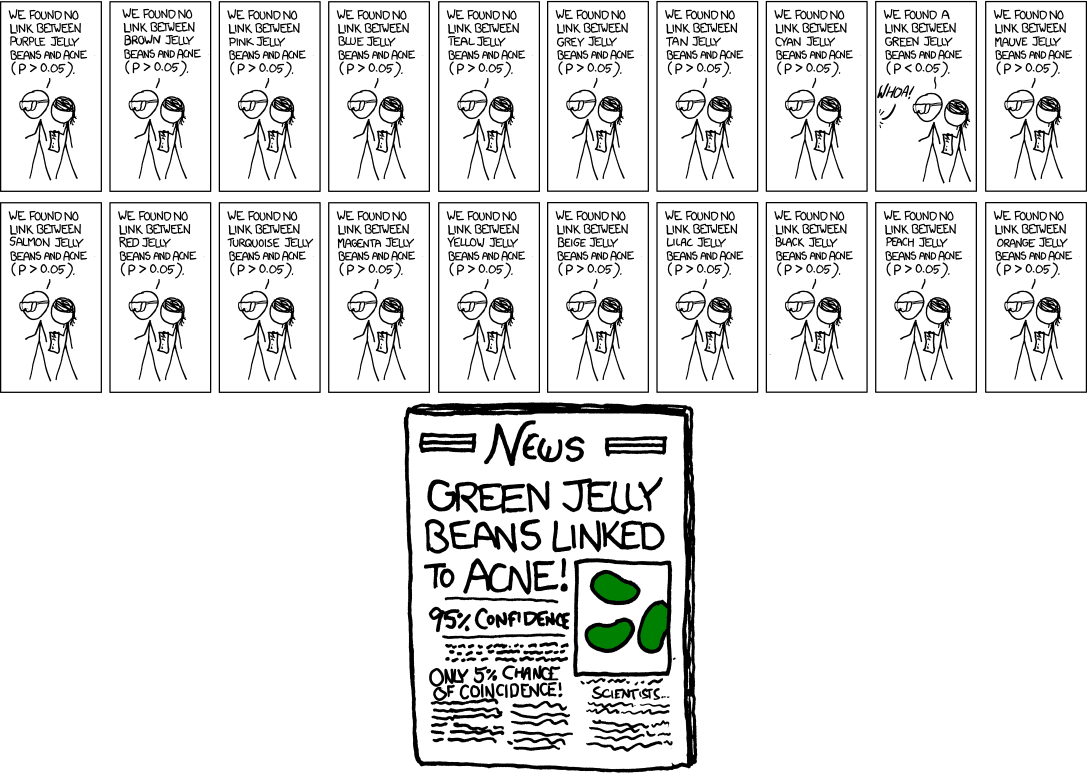
\includegraphics[height=0.8\textheight]{xkcd_significant_crop}
\lfr{Image adapted from \url{https://xkcd.com/882/}}
\end{ftst}

%=====

\begin{ftst}
{Hypothesis Testing}
{p-values, significance and effect sizes}
Statistical $\times$ practical significance: p-values can be made arbitrarily small, if $n$ is big enough;
\vone 
As an example, suppose a test of $H_0: \mu=500$ against a two-sided alternative, with $n=5000, \bar{x}=499,\ s=5$. In this case we would have:

\bitems $t_0 = -14.142$;
\item $p = 1.02\times 10^{-23}$;\eitem
\vone	
Is it really \textit{that} significant?
\end{ftst}

%=====

\begin{ftst}
{Hypothesis Testing}
{p-values, significance and effect sizes}
To ``tell the whole story'' of the experiment, it is necessary to use \textbf{effect size estimators} alongside the tests of statistical significance; 
\vone
While there are whole books on the subject\footnote[3]{\tiny See, for instance, Paul D. Ellis' \textit{The Essential Guide to Effect Sizes}, Cambridge University Press, 2010.}, the main idea is quite simple - to quantify the magnitude of the observed deviation from the null hypothesis.
\vone
Examples of effect size estimators include the simple point estimator for the difference $\bar{x} - \mu_0$, or the dimensionless \textit{d} estimator:

\beqs
d = \frac{\bar{x}-\mu_0}{s}
\eqs

\noindent which quantifies the difference in terms of sample standard deviations.
\vone
\end{ftst}

%=====

\begin{ftstf}
{Hypothesis Testing}
{p-values, effects sizes and confidence intervals}
\begin{block}{}
\centering\textit{Point estimators + confidence intervals quantify the magnitude and accuracy of effects, and must be reported alongside the results of significance testing whenever possible.}
\end{block}
\vhalf
Suppose we are testing $H_0: \mu=50$ against the two-sided alternative hypothesis, with $n=10$ and $\alpha=0.01$. Assume that the population is known to be normal, with unknown variance. We'll use the same data as before:
\vhalf
\begin{rcode}
> t.test(sample, mu = 50, conf.level = 0.99)
(...)
t = -1.5969, df = 9, p-value = 0.1447
alternative hypothesis: true mean is not equal to 50
99 percent confidence interval:
 48.93166 50.36434
sample estimates:
mean of x 
   49.648 
\end{rcode}
\begin{tikzpicture}[remember picture,overlay]
\node[anchor=north east,yshift=12pt,xshift=-5pt] at (current page.north east) {\includegraphics[width=0.2\textwidth]{../Campelo/figs/peas.png}};
\end{tikzpicture}
\end{ftstf}

%=====

\begin{ftst}{Sample size and Type-II error}
{Some considerations}
The probability of Type-II error can be easily (and often wrongly) evaluated \textit{a posteriori}, but its definition \textit{a priori} requires some care;
\vone
Given a desired test, its power is essentially a function of 4 elements:
\bitems Actual size of the difference;
	\item Variability of the observations;
	\item Significance level;
	\item Sample size.
\eitem
\vone
The experimenter generally have very little control over the first two.
\end{ftst}

%=====

\begin{ftst}{Sample size and Type-II error}
{Some considerations}
A strategy for estimating an effective lower bound for the power of a test includes a definition of an \textit{minimally interesting effect} $\delta^*$. 
\vone
This value must be derived from technical and scientific knowledge about the phenomenon or system under experimentation. 
\vhalf
\begin{block}{}
\centering It is essential to have a good understanding of the field in which the experiment will be conducted.
\end{block}
\vhalf
Once $\delta^*$ is defined, the experimenter can obtain an estimate of the variability of observations (e.g., by a pilot study), which can then be used to obtain an approximate power value for the experiment;
\end{ftst}

%=====

\begin{ftst}
{Sample size and Type-II error}
{Some considerations}
Having obtained this estimation of the Type-II error probability, one can run his/her experiment with a better understanding of its ability to detect effects of interest.
\vone
The test will have lower power for differences smaller than $\delta^*$, but these differences are below the minimally interesting effect; any effect greater than $\delta^*$ will result in a higher power for the test;
\vone
This technique can also be used as a way to compute the maximum necessary sample size for the experiment.
\end{ftst}

%=====

\begin{ftstf}
{Sample size and Type-II error}
{Example}
Suppose that on the green peas example we are really interested in detecting negative deviations from the nominal value greater than $1\%$, i.e., $\delta^* = 0.01\times 50 = 0.5$kg. The researcher defines that, for this minimally interesting effect, a test power of $0.85$ is desired. The desired significance is $\alpha = 0.01$.
\vone
The same sample of $n=10$ sacks is used. Assume that you estimated a reasonable standard deviation for this sample as $s=1$kg. From this data, we can compute the power of this test as:
\begin{columns}
\column[T]{0.5\textwidth}
\begin{rcode}
> s <- sd(sample)
> power.t.test(n = 10, 
+        delta = 0.5, 
+        sd = 1, 
+        sig.level = 0.01, 
+        type = "one.sample", 
+        alternative = "one.sided")
\end{rcode}
\column[T]{0.5\textwidth}
\begin{rcode}
One-sample t test power calculation 
n = 10
delta = 0.5
sd = 1
sig.level = 0.01
power = 0.1654013
alternative = one.sided
\end{rcode}
\end{columns}
\begin{tikzpicture}[remember picture,overlay]
\node[anchor=north east,yshift=12pt,xshift=-5pt] at (current page.north east) {\includegraphics[width=0.2\textwidth]{../Campelo/figs/peas.png}};
\node[anchor=south east,yshift=31pt,xshift=-75pt] at (current page.south east) {\footnotesize\color{red}$\boldsymbol{\longleftarrow}$};
\end{tikzpicture}
\end{ftstf}

%=====

\begin{ftstf}
{Sample size and Type-II error}
{Example}
What is the smallest sample size needed to obtain the desired power of $0.85$?
\vhalf
\begin{rcode}
> power.t.test(power = 0.85, delta = 0.5, sd = 1, sig.level = 0.01,
               type = "one.sample", alternative = "one.sided")

One-sample t test power calculation 
n = 47.98044
delta = 0.5
sd = 1
sig.level = 0.01
power = 0.85
alternative = one.sided
\end{rcode}
\vhalf
We need at least 48 observations to detect a $-5g\ (1\%)$ or larger deviation on the mean weight of the green peas packages with a power level of $0.85$.
\begin{tikzpicture}[remember picture,overlay]
\node[anchor=north east,yshift=12pt,xshift=-5pt] at (current page.north east) {\includegraphics[width=0.2\textwidth]{../Campelo/figs/peas.png}};
\node[anchor=south east,yshift=140pt,xshift=-182pt] at (current page.south east) {\footnotesize\color{red}$\mbf{\longleftarrow}$ \textbf{(round this value up)}};
\end{tikzpicture}
\end{ftstf}


\begin{ftst}
{Bibliography}
{\ }
\scriptsize

\benums D.C. Montgomery, G.C. Runger, \textit{Applied Statistics and Probability for Engineers}, Ch. 9.\\5th ed., Wiley, 2010. 
\item J.T. Mordkoff (2011), \textit{The assumption(s) of normality} - \url{http://goo.gl/Z3w8ku}

\item A. Reinhart, \textit{Statistics Done Wrong: the woefully complete guide} - {\tiny\url{http://www.statisticsdonewrong.com}}
\item W. Thalheimer and S. Cook, \textit{How to calculate effect sizes from published research articles: A simplified methodology} - {\tiny\url{http://goo.gl/c0g1oK}}
\item E. Ernst and S. Singh, \textit{Trick or Treatment}, Norton \& Company, 2009.
\eenum
\end{ftst}

%=====

\begin{ftstf}{About this material}{Conditions of use and referencing}
\centering\footnotesize This work is licensed under the Creative Commons CC BY-NC-SA 4.0 license\\(Attribution Non-Commercial Share Alike International License version 4.0).\\
\vhalf
\url{http://creativecommons.org/licenses/by-nc-sa/4.0/}\\
\vone
\footnotesize Please reference this work as:\\
\footnotesize \flushleft Felipe Campelo (2015), \textit{Lecture Notes on Design and Analysis of Experiments}.\\Online: {\scriptsize\url{https://github.com/fcampelo/Design-and-Analysis-of-Experiments}}\\
Version 2.11, Chapter 5; Creative Commons BY-NC-SA 4.0.\\

\begin{Verbatim}[fontsize=\tiny]
    @Misc{Campelo2015-01,
      title={Lecture Notes on Design and Analysis of Experiments},
      author={Felipe Campelo},
      howPublished={\url{https://github.com/fcampelo/Design-and-Analysis-of-Experiments}},
      year={2015},
      note={Version 2.11, Chapter 5; Creative Commons BY-NC-SA 4.0.},
    }
\end{Verbatim}

\begin{tikzpicture} [remember picture,overlay]
\node[anchor=south,yshift=0pt] at (current page.south){ \includegraphics[width=.2\textwidth]{../Campelo/figs/CCSomerights.png}};
\end{tikzpicture}
\end{ftstf}


\end{document}
